\section{Auswertung}
\label{sec:Auswertung}

Die gemessenen Temperaturen $T_1$ und $T_2$, sowie die Drücke
$p_a$ und $p_b$ und die Leistungsaufnahme des Kompressors
zu verschiedenen Zeiten $t$ sind in Tabelle \ref{tab1}
dargestellt.
\begin{table}\caption{Der maximale Drehimpuls $L$, der Gesamtspin $S$ und der Gesamtdrehimpuls $J$ ergeben sich zum Landé-Faktor $g_\text{J}$ für die vier verschiedenen Elemente.}
\label{tab1}
\centering
\sisetup{round-mode = places, round-precision=2, round-integer-to-decimal=true}
\begin{tabular}{S[]S[]S[]S[]} 
\toprule
{$L$} & {$S$} & {$J$} & {$g_\text{J}$}\\
\midrule
5.0 & 1.0 & 4.0 & 0.8\\
0.0 & 3.5 & 3.5 & 2.0\\
6.0 & 1.5 & 4.5 & 0.7272727272727273\\
5.0 & 2.5 & 7.5 & 1.3333333333333333\\
\bottomrule
\end{tabular}\end{table}

\subsection{Temperaturverläufe}
%a & b) 
Die Temperaturverläufe der beiden Reservoire sind in Abbildung
\ref{fig:plot1} zu sehen.

\begin{figure} %Funktion in die Abbildung schreiben?
    \centering
    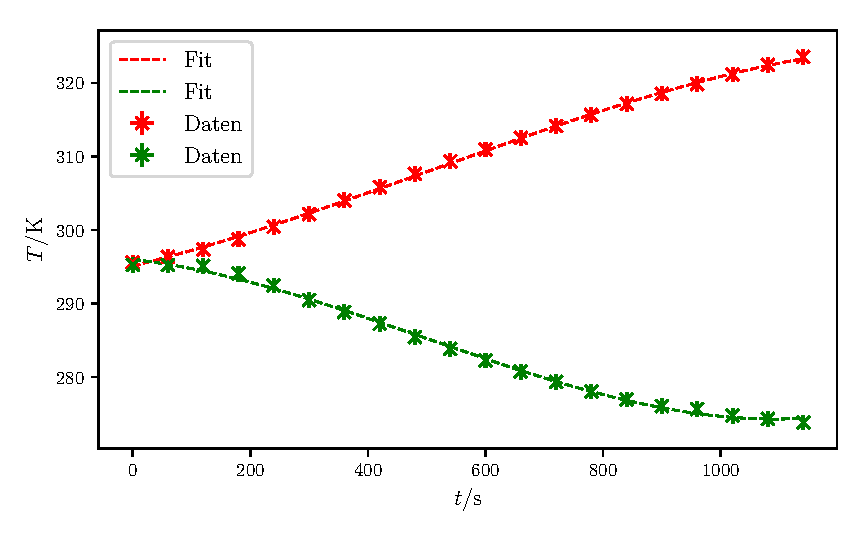
\includegraphics[width=14cm, height=10cm]{build/plot1.pdf}
    \caption{Temperaturverläufe. Es sind jeweils die Daten und ein Fit dargestellt.
    Die rote Kurve stellt die Temperatur in Reservoir x dar. Die grüne Kurve stellt 
    die Temperatur in Reservoir y dar. Dabei wird die Temperatur
    durch ein Polynom dritten Grades dargestellt: $T(t) = At^3+Bt^2+Ct+D$. 
    Die Fitparameter der Kurve der Temperatur im ersten Reservoir sind $A_1=\num{-1.20(17)e-8}$,
    $B_1=\num{1.83(30)e-5}$, $C_1=\num{1.95(14)e-2}$ und $D_1=\num{295.11 \pm 0.18}$.
    Die Fitparameter der Kurve der Temperatur im zweiten Reservoir sind $A_2=\num{2.61(30)e-8}$,
$B_2=\num{-3.87(52)e-5}$, $C_2=\num{-0.87(25)e-2}$ und $D_2=\num{295.99 \pm 0.32}$.} %hier ist irgendwas falsch. Der Fehler war, dass du beim ersten D1 SI statt num geschrieben hast. Dann hatte er keine Einheit und konnte das nicht. :)

    \label{fig:plot1}
\end{figure}

%c)
Die Differentialquotienten $\frac{dT}{dt}$ für vier verschiedene Temperaturen
sind im Folgenden zu sehen. Es werden die Temperaturen
\begin{align*}
    T_1 &= \SI{1}{\degreeCelsius} &= \SI{274.15}{\kelvin} \\ %celsius geht nicht, degreeCelsius auch nicht, keine Ahnung warum. Bei den oberen beiden ging es. Du hattest bei T3 und T4 num stehen :D
    T_2 &= \SI{5}{\degreeCelsius} &= \SI{278.15}{\kelvin}\\
    T_3 &= \SI{10}{\degreeCelsius} &= \SI{283.15}{\kelvin}\\
    T_4 &= \SI{15}{\degreeCelsius} &= \SI{288.15}{\kelvin}
\end{align*}
betrachtet.
%Das schon in die Theorie?:
Dabei ist \eqref{eqn:} %Gleichung einfügen (Polynom)
die Ableitung der Funktion der Temperatur $T(t)$.
Für $\frac{dT_1}{dt}$ folgt:
\begin{align*}
    dT_{1,1}(1) &= \num{0.0216 \pm 0.0015} \\
    dT_{1,2}(5) &= \num{0.0272 \pm 0.0023} \\
    dT_{1,3}(10) &= \num{0.028 \pm 0.004} \\
    dT_{1,4}(15) &= \num{0.023 \pm 0.007} %schöner angeben? Einheit? Einheit müsste K/Sekunde sein
\end{align*}
Für $\frac{dT_2}{dt}$ gilt:
\begin{align*}
    dT_{2,1}(1) &= \num{-0.0130 \pm 0.0026} \\ %0 oder 1 Grad? Lieber in Kelvin angeben? Wie meinst du das mit 0 oder 1 Grad? hab eigentlich alles in Kelvin berechnet, dachte ich.  
    dT_{2,2}(5) &= \num{-0.025 \pm 0.004} \\
    dT_{2,3}(10) &= \num{-0.027 \pm 0.007} \\
    dT_{2,4}(15) &= \num{-0.015 \pm 0.012}
\end{align*}

%d)
\subsection{Bestimmung der Güteziffern}
%c_w angeben
Die Wärmekapazität der Kupferschlange und des Eimers beträgt
\begin{equation*}
    m_\text{k} c_\text{k} = \SI{750}{\joule\per\kelvin}.
\end{equation*}
Die realen Güteziffern für die vier Temperaturen werden mittels
Gleichung \eqref{eqn:güteziffer} berechnet. %Stimmt das?
Die idealen Güteziffern werden mit Gleichung \eqref{eqn:ideal} %Stimmt das?
bestimmt.
Beide Größen sind in Tabelle \ref{tabsolution1} jeweils
gegenübergestellt.
\begin{table}
\caption{Die Ergebnisse für die realen und idealen Gütewerte für die vier verschiedenen Temperaturwerte.}
\label{tabsolution1}
\centering
\begin{tabular}{S[table-format=1.2]  
        @{${} \pm{}$}
        S[table-format=1.2]
        @{$  $}
        S[table-format=5.1]
        @{${} \pm{}$}
    S[table-format=3.1]}
\toprule
   \multicolumn{2}{c}{$\nu_\text{real}$} &\multicolumn{2}{c}{$\nu_\text{ideal}$}\\
\midrule
    0.64 & 0.05 & 270.0 & 350.0\\
    0.67 & 0.06 & 25.8 & 3.1\\
    0.68 & 0.1 & 10.8 & 0.5\\
    0.54 & 0.16 & 7.5 & 0.23\\
\bottomrule
\end{tabular}\end{table}


%e)
\subsection{Bestimmung des Massendurchsatzes}
Das im Versuch verwendete Gas ist Dichlordifluormethan.
Die Verdampfungswärme $L$ des Gases wird durch die Dampfdruck-Kurve
in Abb. \ref{fig:plot2} bestimmt. %wie? In V203 gucken
Die Wertepaare des Drucks $p$ und der Temperatur $T$, die zur
Darstellung der Dampfdruck-Kurve nötig sind, befinden sich in
Tabelle \ref{tab2}. 
\begin{table}\caption{Das Verhältnis des magnetischen Feldes durch die Beschleunigungsspannung aufgetragen gegen die Höhe.}
\label{tab2}
\centering
\sisetup{round-mode = places, round-precision=2, round-integer-to-decimal=true}
\begin{tabular}{S[]S[]S[]} 
\toprule
{$B_1 / \si{\henry}$} & {$B_2 / \si{\henry}$} & {$\frac{D}{(L^2 + D^2)} / \si{\per\meter}$}\\
\midrule
0.0 & 0.0 & 0.0\\
3.5649278338607584e-07 & 3.862005153349155e-07 & 0.29289724188430566\\
8.912319584651897e-07 & 8.912319584651897e-07 & 0.5827222842713544\\
1.4259711335443034e-06 & 1.396263401595464e-06 & 0.8665094112549946\\
1.9250610302848096e-06 & 1.8418793808280586e-06 & 1.1414982164090373\\
2.3885016486867084e-06 & 2.3172030920094934e-06 & 1.4052180429996723\\
2.923240823765822e-06 & 2.822234535139767e-06 & 1.6555530006898145\\
3.4223307205063282e-06 & 3.3272659782700412e-06 & 1.8907846756403912\\
\bottomrule
\end{tabular}\end{table}
\begin{figure}
    \centering
    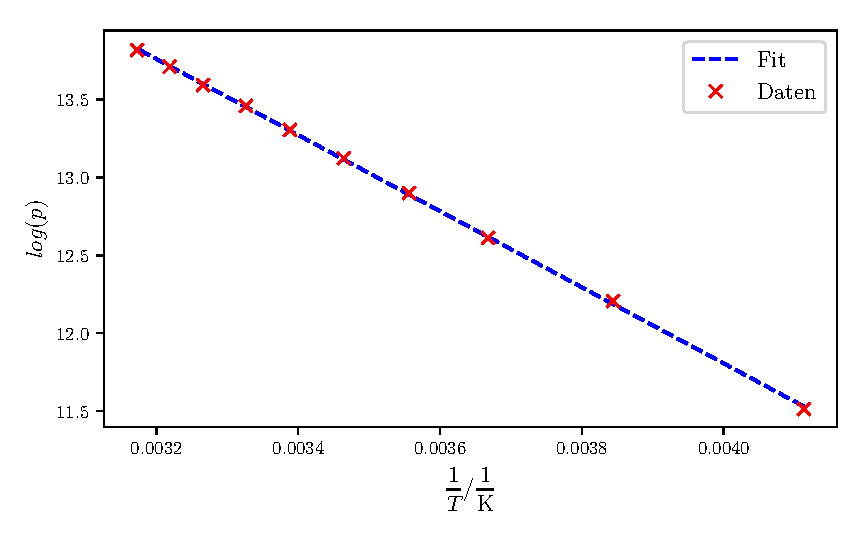
\includegraphics[width=14cm, height=10cm]{build/plot2.pdf}
    \caption{Dampfdruck-Kurve.}
    \label{fig:plot2}
\end{figure}
Die Verdampfungswärme ist durch eine Ausgleichsrechnung somit %wie kommt man darauf?
\begin{equation*}
    L = \SI{-2.032(011)e4}{}. %Einheit? Einheiten stehen alle auf dem heiligen Zettel :D müsste Pa*s sein oder so, wenn ich mich richtig erinnere.
\end{equation*}
Die Massendurchsätze ergeben sich damit mit Gleichung \eqref{eqn:massendurchsatz} zu %was ist Q_2?
\begin{align*}
    m_1 &= \SI{0.0032 \pm 0.0006}{} \\
    m_2 &= \SI{0.0060 \pm 0.0010}{} \\
    m_3 &= \SI{0.00103 \pm 0.00029}{} \\
    m_4 &= \SI{0.0006 \pm 0.0005}{}. %Einheit? Anders angben? kg/Sekunde vermutlich. Ich hatte die auch nur m1 genannt. Eigentlich ist das dm/delta*t oder so.
\end{align*}

%f)
\subsection{Bestimmung der mechanischen Kompressorleistung}
Dichlordifluormethan hat bei den Werten
\begin{align*}
    T &= \SI{273.15}{\kelvin} \\
    p &= \SI{e5}{\pascal} \\
    \kappa &= \num{1.14}
\end{align*}
die Dichte 
\begin{equation*}
    \rho_0 = \SI{5.51}{\gram\per\liter},
\end{equation*}
die mit Gleichung \eqref{eqn:dichte} berechnet werden kann.
Die mechanischen Kompressorleistungen für die vier Temperaturen
ergeben sich mit Gleichung \eqref{eqn:nmech}
zu den in Tabelle \ref{tabsolution2} stehen Werten.
\begin{table}\caption{Die Ergebnisse für die mechanische und die elektrische Leistung für die vier verschiedenen Temperaturwerte.}
\label{tabsolution2}
\centering
\sisetup{round-mode = places, round-precision=2, round-integer-to-decimal=true}
\begin{tabular}{S[]S[]} 
\toprule
{\nu_\text{real}} & {\nu_\text{ideal}}\\
\midrule
 135 \pm 32 & 165\\
 160 \pm 40 &  200\\
 50 \pm 70 & 208\\
 310 \pm 140 & 212\\
\bottomrule
\end{tabular}\end{table}
 %Für die el. Leistung ist das kein Ergebnis
